\tikzset{
	main/.style={black, line width=0.4mm, opacity=1},
	second/.style={gray, opacity=5},
	arrow/.style={-latex, shorten >=1ex, shorten <=1ex, bend angle=45}
}
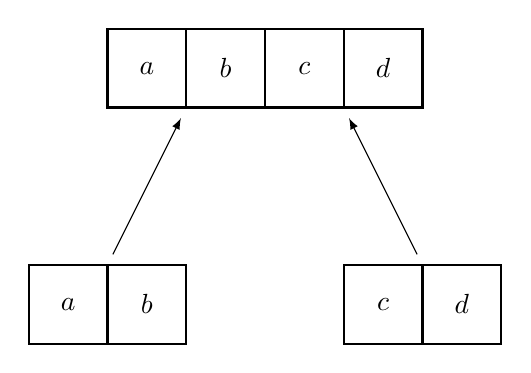
\begin{tikzpicture}
\node (rect) at (1,0) [draw,thick,minimum width=1cm,minimum height=1cm]  {$a$};
\node (rect) at (2,0) [draw,thick,minimum width=1cm,minimum height=1cm]  {$b$};
\node (rect) at (3,0) [draw,thick,minimum width=1cm,minimum height=1cm]  {$c$};
\node (rect) at (4,0) [draw,thick,minimum width=1cm,minimum height=1cm]  {$d$};

\node (rect) at (0,-3) [draw,thick,minimum width=1cm,minimum height=1cm] {$a$};
\node (rect) at (1,-3) [draw,thick,minimum width=1cm,minimum height=1cm] {$b$};

\node (rect) at (4,-3) [draw,thick,minimum width=1cm,minimum height=1cm] {$c$};
\node (rect) at (5,-3) [draw,thick,minimum width=1cm,minimum height=1cm] {$d$};


\draw [arrow]  (0.5,-2.5) to (1.5,-0.5) ;
\draw [arrow]  (4.5,-2.5) to (3.5,-0.5) ;

\end{tikzpicture}